\subsection{Terrain editing}
The player has three "terrain modifiers", represented with pickaxe symbols, at their disposal.
Using the terrain modifier, the player can edit the game's landscape by building new structures or digging in the ground.
As an example of the "creation capabilities", we show in \autoref{fig:hyper-logo} how the letters making up the game's name could be created inside the game.
\begin{figure}[!htb]
    \centering
    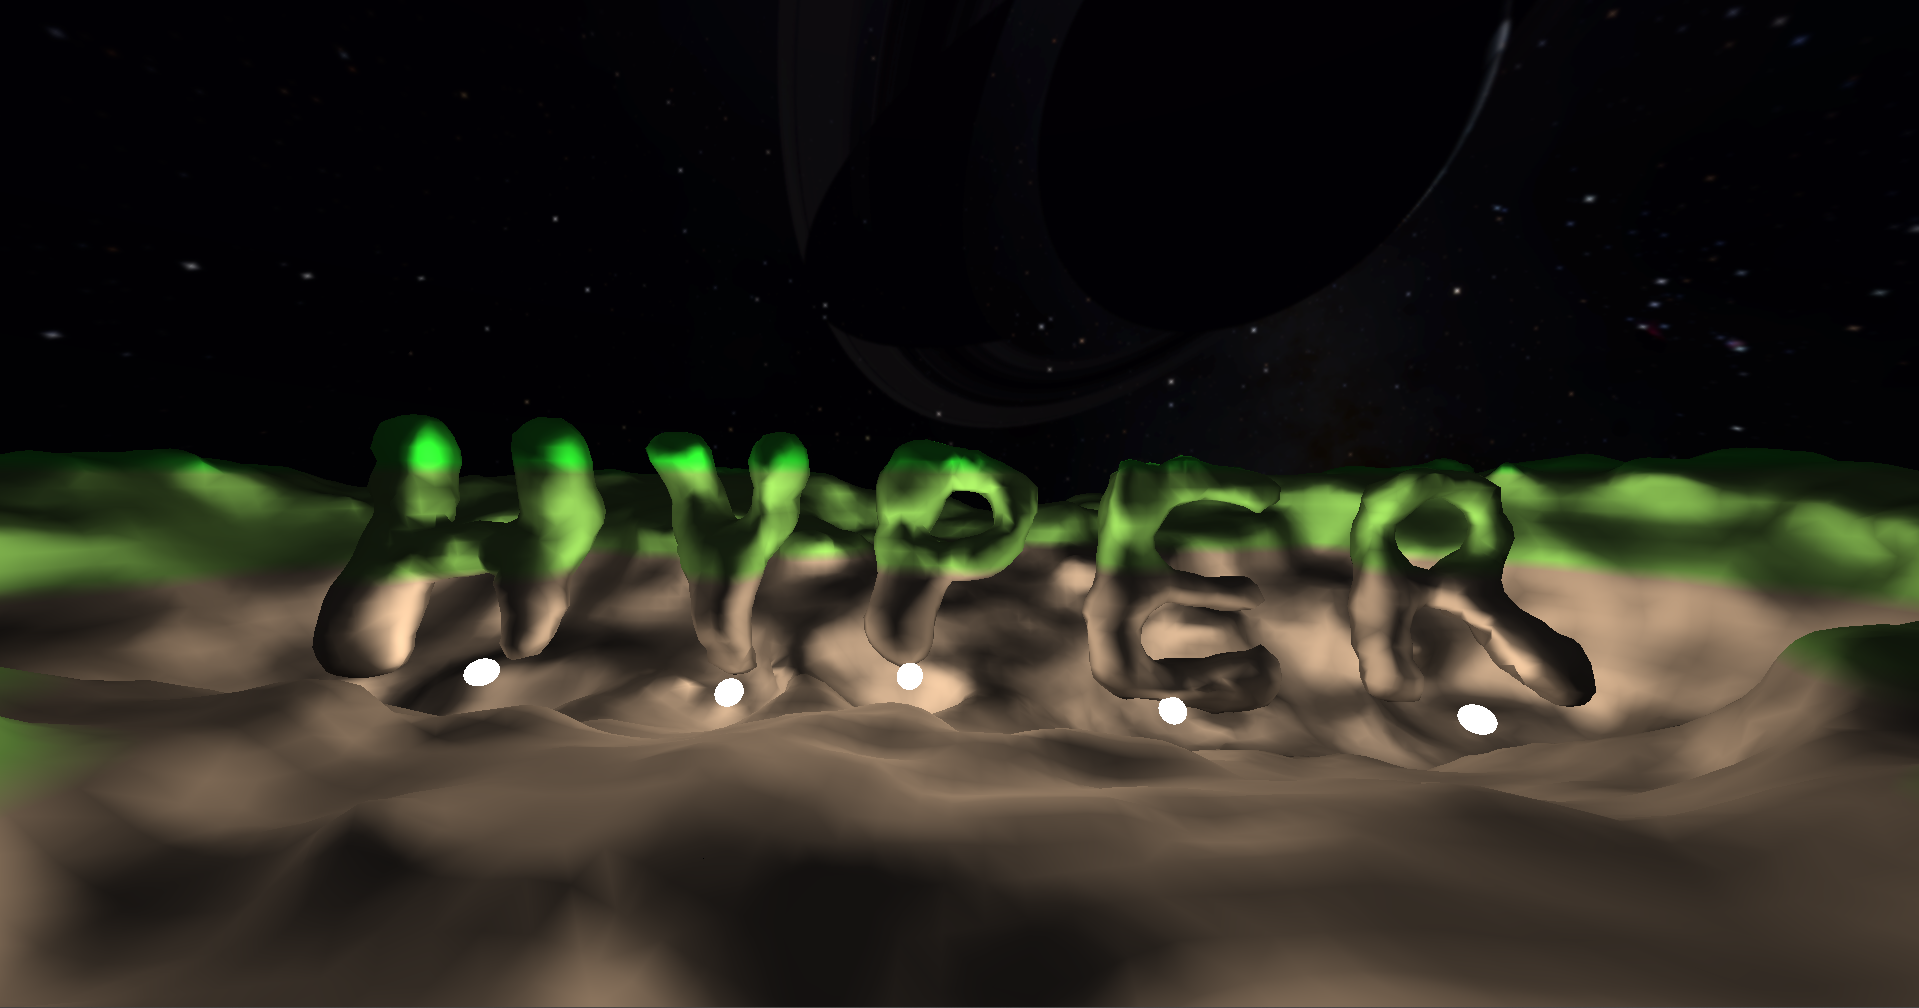
\includegraphics[width=0.8\textwidth]{chapters/results/sections/gameplay/resources/hyper-logo-night-2.png}
    \caption{The letters of the word "Hyper" created in the game}
    \label{fig:hyper-logo}
\end{figure}

As mentioned before the terrain modifiers can also be used for carving in the terrain.
To illustrate that, in \autoref{fig:tunnel-under-hill} we show a tunnel that was dug through a hill.
\begin{figure}[!htb]
    \centering
    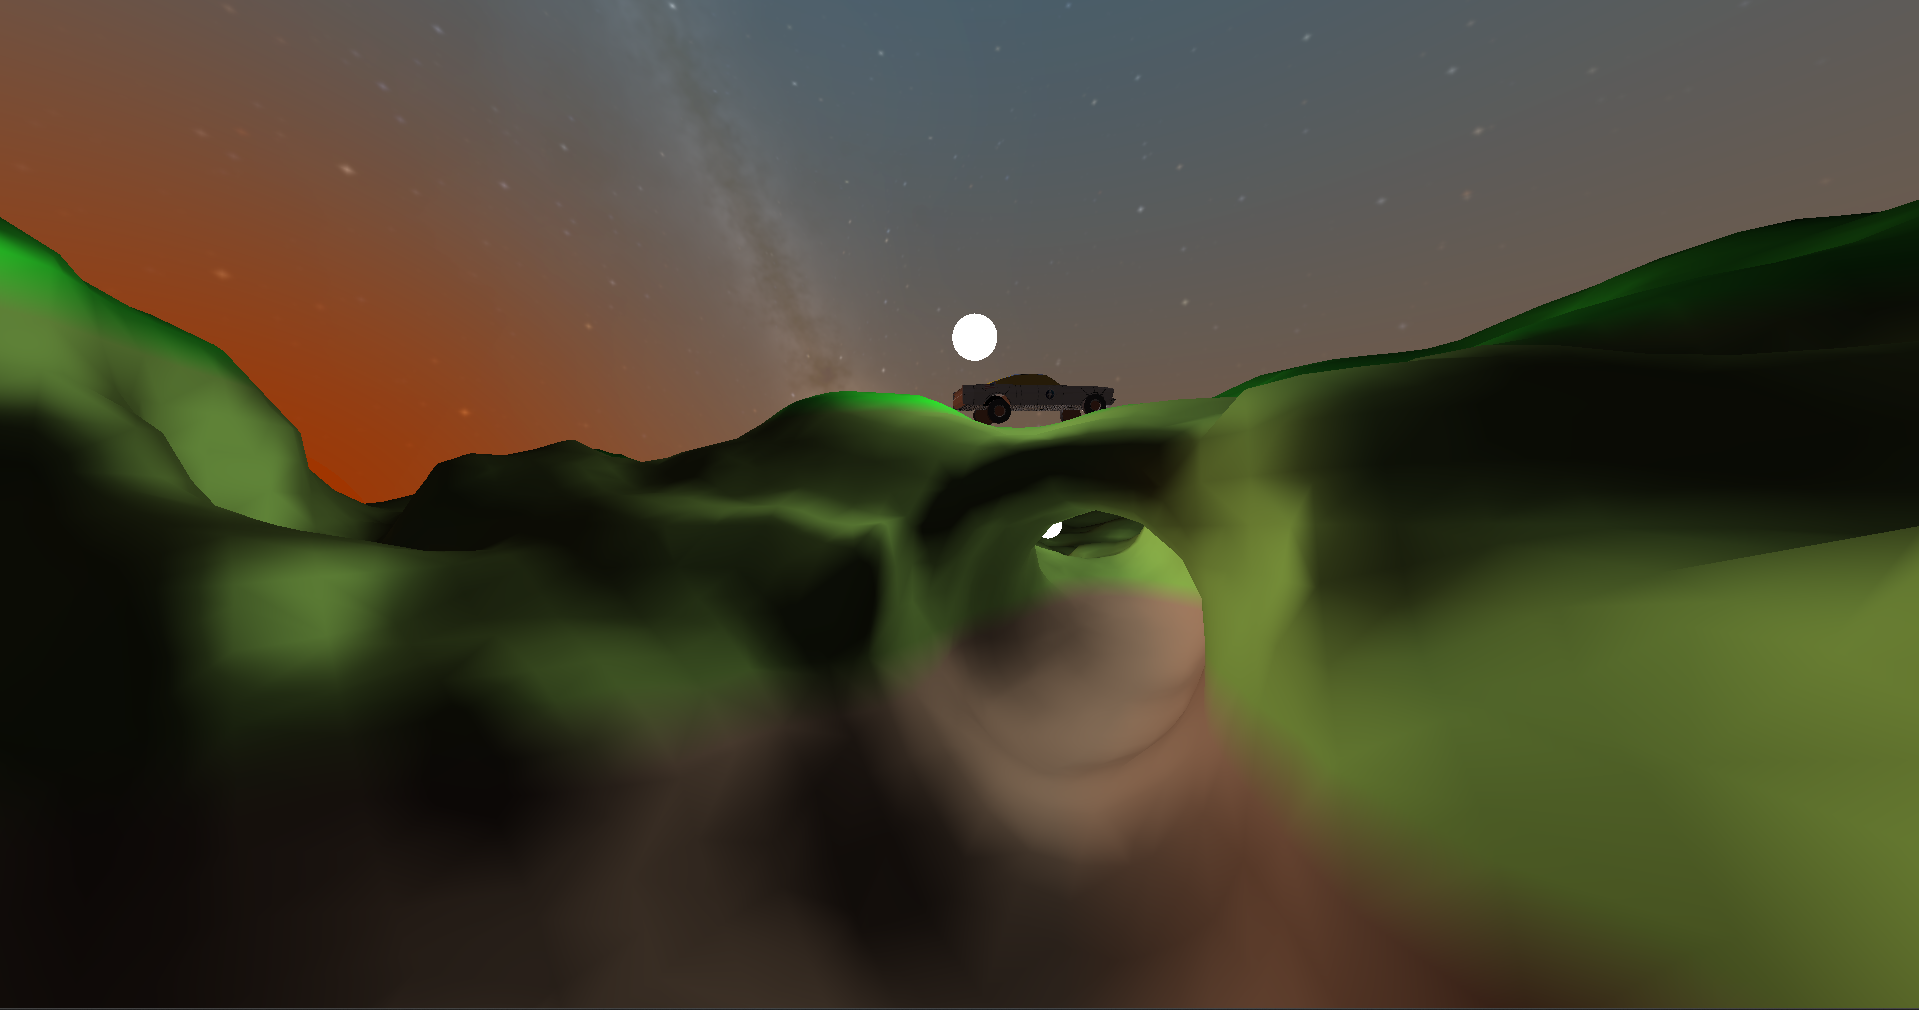
\includegraphics[width=0.8\textwidth]{chapters/results/sections/gameplay/resources/tunnel-with-car.png}
    \caption{Tunnel dug under a hill}
    \label{fig:tunnel-under-hill}
\end{figure}
